% Paper template for TAR 2016
% (C) 2014 Jan Šnajder, Goran Glavaš, Domagoj Alagić, Mladen Karan
% TakeLab, FER

\documentclass[10pt, a4paper]{article}

\usepackage{tar2016}

\usepackage[utf8]{inputenc}
\usepackage[pdftex]{graphicx}
\usepackage{booktabs}
\usepackage{amsmath}
\usepackage{amssymb}
\usepackage{float}
\usepackage{graphicx}
\usepackage{caption}
\usepackage{subcaption}

\graphicspath{{img/}}

\title{Semantic Textual Similarity using deep learning}

\name{Bruno Gavranovic, Neven Miculinic, Stipan Mikulic}

\address{
University of Zagreb, Faculty of Electrical Engineering and Computing\\
Unska 3, 10000 Zagreb, Croatia\\
\texttt{\{bruno.gavranovic,neven.miculinic,stipan.mikulic\}@fer.hr}\\
}


\abstract{
In this paper we present our work on Semantic Textual Similarity (STS) problem during Text analysis and retrival (TAR) class at FER.
STS measures semantic similarity between two sentences.
We use two approaches: an SVM model with feature preprocessing and a deep learning model trained on a language modelling task.
Datasets were obtained using human annotators and their average semantic similarity score is given.
We use both Pearson and Spearman correlation coefficient in our analysis and achieve 1.000, and 1.000 on our test set respectively.
}

\begin{document}

\maketitleabstract

\section{Introduction}

\begin{verbatim}
Two dogs play in the grass.
Two dogs playing in the snow.
\end{verbatim}
At the heart of STS, semantic textual similarity, is assigning numerical score on two text similarity. By text, it could mean full document, paragraph, or in this paper's case only one sentence. Beginning quote showcases one such sentance pairs, where human annotators rated 2.8 semantically similar on 0-5 scale, where 0 mean full semantic dissimilarity, and 5 full equivalence with various shades in between. Full score semantics you can read in table~\ref{tab:sts-score}
STS developed system and techniqus have many further applications, transfer learning of sorts. Machine translation(MT), Summarization, Generation and Question Answering(QA) are some of them. Often new techniques invented in STS context generlize to earlier mentioned domains, as well as NLP fiels as a whole.


\begin{table*}
\caption{STS score description, adapted from~\citep{agirre2016semeval}}
\label{tab:sts-score}
\begin{center}
\begin{tabular}{llr}
\toprule
Score & Explanation\\
\midrule
5 & \textit{Two sentences are completely equivalent}\\
& The bird is bathing in the sink\\
& Birdie is washing itself in the water basin.\\
\midrule
4 & \textit{The two sentences are mostly equivalent, but some unimportant details differ}\\
& In May 2010, the troops attempted to invade
Kabul. \\
& The US army invaded Kabul on May 7th last
year, 2010.\\
\midrule
3 & \textit{The two sentences are roughly equivalent, but some important information differs/missing.}\\
& John said he is considered a witness but not a
suspect.\\
& ``He is not a suspect anymore.'' John said.\\
\midrule
2 & \textit{The two sentences are not equivalent, but share some details.} \\
&They flew out of the nest in groups. \\
&They flew into the nest together. \\
\midrule
1 & \textit{The two sentences are not equivalent, but are on the same topic.}\\
& The woman is playing the violin.\\
& The young lady enjoys listening to the guitar.\\
\midrule
0 & \textit{The two sentences are completely dissimilar.}\\
& John went horse back riding at dawn with a whole group of friends.\\
& Sunrise at dawn is a magnificent view to take in if you wake up early enough for it.\\
\bottomrule
\end{tabular}
\end{center}
\end{table*}

\section{Related work}

STS has short and fruitful history, one with many ideas flying around. In its current form it appeared in 2012, on SemVal~\citep{agirre2012semeval} as task 6.  In 2012, the best system~\citep{bar2012ukp} used lexical similarity and Explicit Semantic Analysis(ESA)~\citep{gabrilovich2007computing}. Following year Latent Semantic Analysis(LSA)~\citep{deerwester1990indexing} model~\citep{han2013umbc} with additional external information sources, WordNet and n-gram matching technique.

Following two years~\citep{sultan2014dls} and~\citep{sultan2015dls} dominate the competition with new algorithm -- they align the words between new sentences. Other notable approaches come from logic side, its representative paper being~\citep{beltagy2014probabilistic}.

\section{Extent of the paper}

Our contribution consists of implementation of two machine learning models: SVM model and a deep learning model.

\subsection{Data analysis}
We used dataset from SemEval 2017 
Task 1\footnote{http://alt.qcri.org/semeval2017/task1/}. 
The dataset has 250 instances. Each instance consists of two sentences and our tash is to predict semantic similarity between them. In order to get some deeper insights on data we did some minor data analysis. We got to conclusion that we are dealing with very short text. Also, we concluded that the smaller difference between lengths of sentences is, the more similar they are. This can be seen clearer on following plots.

\begin{table}
\caption{Stats about lengths of sentences}
\label{tab:narrow-table}
\begin{center}
\begin{tabular}{cll}
\toprule
& Without stopwords & With stopwords \\
\midrule
Sentence length & 33.004 & 43.838 \\
Tokens in sentence & 5.488 & 8.702 \\
\bottomrule
\end{tabular}
\end{center}
\end{table}

\begin{figure*}[t!]
    \centering
    \begin{subfigure}[t]{0.5\textwidth}
        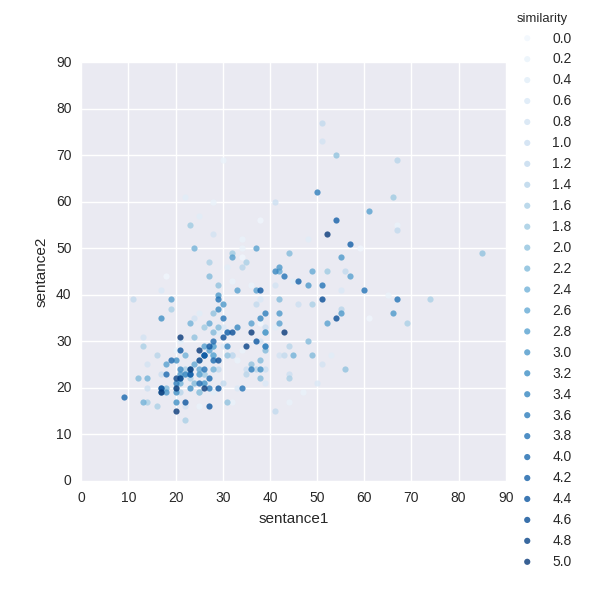
\includegraphics[width=\columnwidth]{sen_len_no_stop.png}
		\caption{Sentence lengths without stopwords}
    \end{subfigure}%
    ~ 
    \begin{subfigure}[t]{0.5\textwidth}
        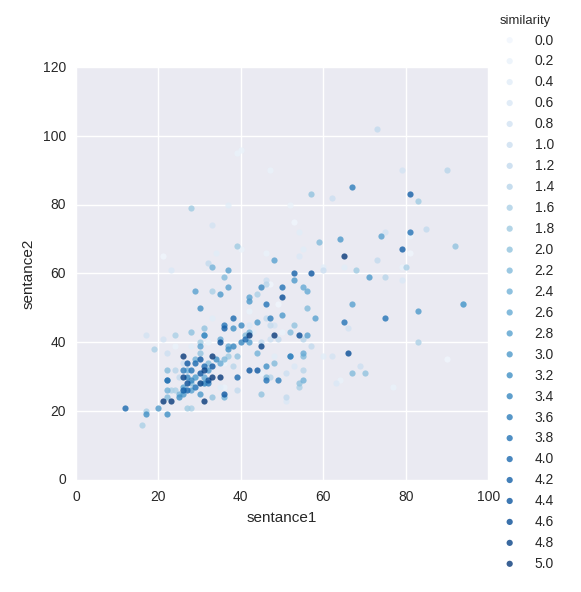
\includegraphics[width=\columnwidth]{sen_len_with_stop.png}
		\caption{Sentence lengths with stopwords}
    \end{subfigure}
    ~ 
    \caption{Sentence length stats}
\end{figure*}

\begin{figure*}[t!]
    \centering
    \begin{subfigure}[t]{0.47\textwidth}
		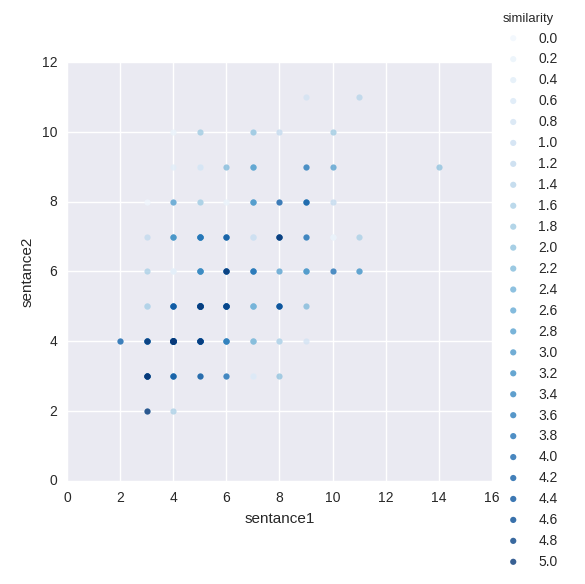
\includegraphics[width=\columnwidth]{tokens_no_stop.png}
		\caption{Number of tokens without stopwords}
    \end{subfigure}
    ~ 
    \begin{subfigure}[t]{0.49\textwidth}
		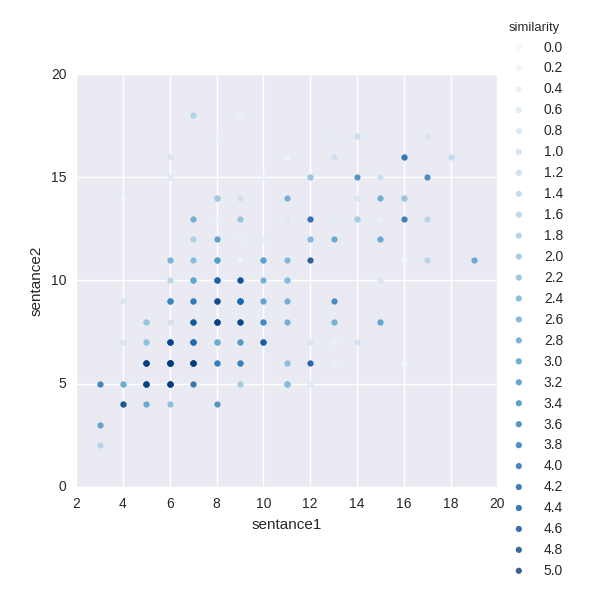
\includegraphics[width=\columnwidth]{tokens_with_stop.png}
		\caption{Number of tokens with stopwords}
    \end{subfigure}
    ~ 
    \caption{Number of tokens stats}
\end{figure*}

%\begin{figure}[h]
%\begin{center}
%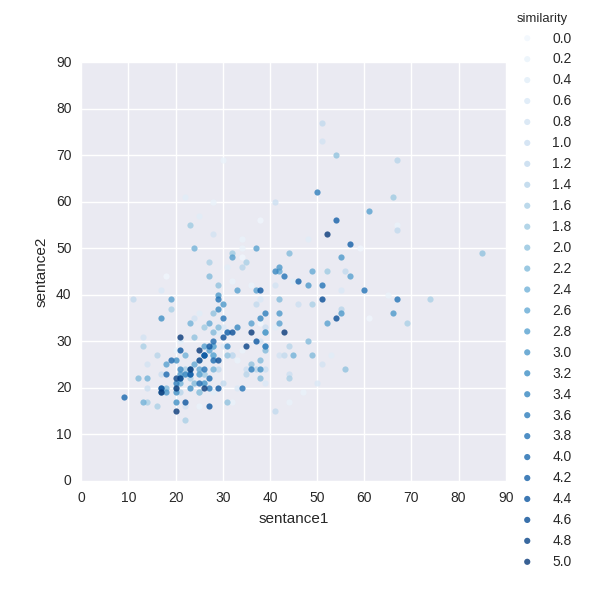
\includegraphics[width=\columnwidth]{sen_len_no_stop.png}
%\caption{Sentence lengths without stopwords}
%\label{fig:lstm_2nd_layer}
%\end{center}
%\end{figure}
%
%\begin{figure}[h]
%\begin{center}
%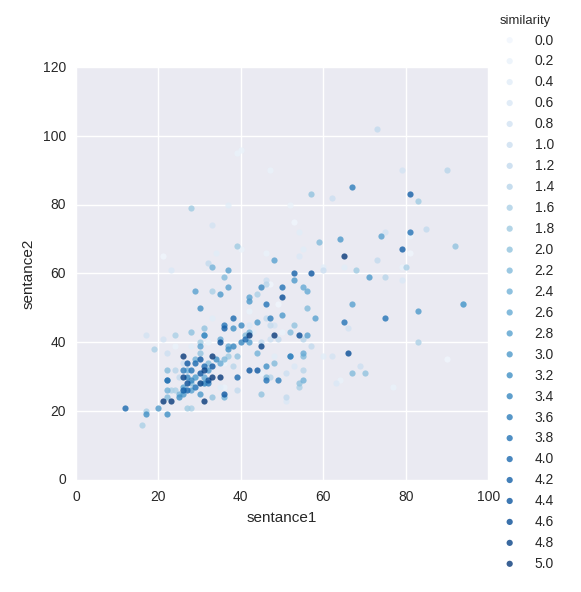
\includegraphics[width=\columnwidth]{sen_len_with_stop.png}
%\caption{Sentence lengths with stopwords}
%\label{fig:lstm_2nd_layer}
%\end{center}
%\end{figure}
%
%\begin{figure}[h]
%\begin{center}
%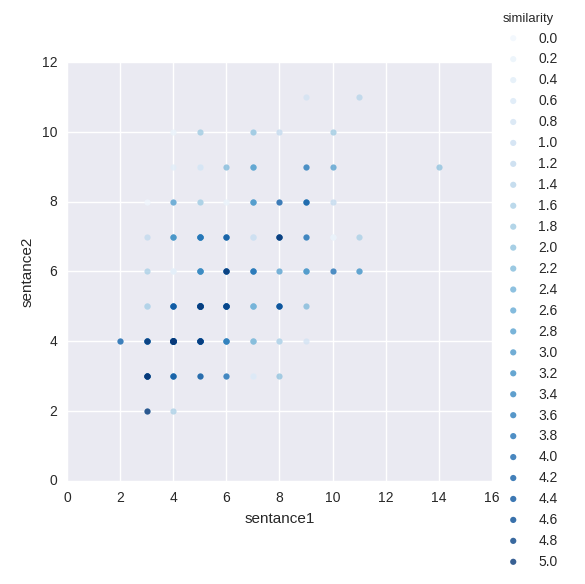
\includegraphics[width=\columnwidth]{tokens_no_stop.png}
%\caption{Number of tokens without stopwords}
%\label{fig:lstm_2nd_layer}
%\end{center}
%\end{figure}
%
%\begin{figure}[h]
%\begin{center}
%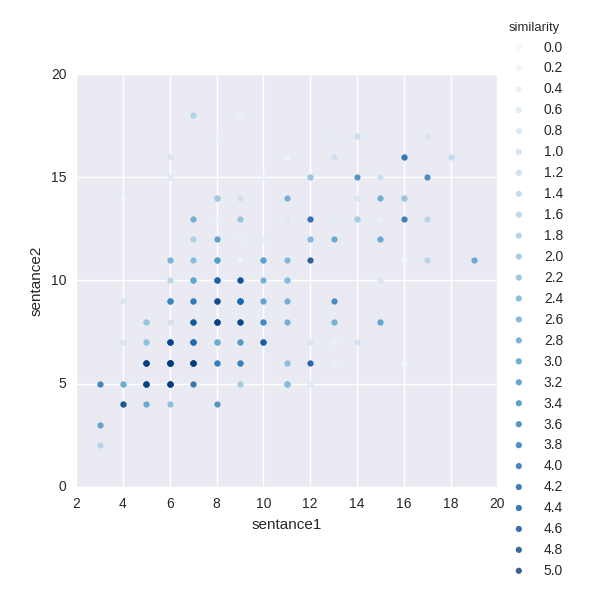
\includegraphics[width=\columnwidth]{tokens_with_stop.png}
%\caption{Number of tokens with stopwords}
%\label{fig:lstm_2nd_layer}
%\end{center}
%\end{figure}

\newpage
\subsection{SVM}

\subsubsection{Features}
All of the features we used are from \citep{Saric2012TakeLabSF} paper.
\paragraph{Ngram Overlap \\}
Let S1 and S2 be the sets of consecutive ngrams in the first and the second sentence, respectively. The ngram overlap is computed for unigrams, bigrams, and trigrams. It is defined as follows:
\begin{equation}\label{eq:ngo}
ngo(S_1, S_2) = 2 \cdot \bigg( \frac{|S_1|}{|S_1 \cap S_2|}+\frac{|S_2|}{|S_1 \cap S_2|}\bigg)^{-1}
\end{equation}

The ngram overlap is the harmonic mean of the degree
to which the second sentence covers the first
and vice versa.\citep{Saric2012TakeLabSF}

\paragraph{WordNet-Augmented Word Overlap \\}
In order to determine some semantical meaning from words we define the WordNet augmented coverage $ PWN(\cdot, \cdot) $:
\begin{equation}\label{eq:pwn}
P_{WN}(S_1, S_2) = \frac{1}{|S_2|} \sum_{w \in S_1} score(w, S_2)
\end{equation}

\begin{equation}\label{eq:pwn-score}
score(w, S) = \begin{cases}
1 & \text{if $w \in S $}\\
\max\limits_{w^{\rq} \in S} sim(w, w^{\rq}) & \text{otherwise}
\end{cases}
\end{equation}

where $sim(\cdot, \cdot)$ represents the WordNet path length
similarity. The WordNet-augmented word overlap
feature is defined as a harmonic mean of
$PWN(S_1, S_2)$ and $PWN(S_2, S_1)$.\citep{Saric2012TakeLabSF}


\paragraph{Weighted Word Overlap \\}
We define information contente measure to give some words more importance:
\begin{equation}\label{eq:inf-content}
ic(w) = ln \frac{\sum_{w^{\rq} \in C} freq(w^{\rq}) }{freq(w)}
\end{equation}
where C is the set of words in the corpus and
freq(w) is the frequency of the word w in the corpus. Since we got very small dataset we used \emph{nltk brown} dataset to calculate word frequency distribution.
The weighted word coverage of the second sentence by the first sentence is given by:
\begin{equation}\label{eq:wwc}
wwc(S_1, S_2) = \frac{\sum_{w \in S_1 \cap S_2} ic(w)}{\sum_{w^{\rq} \in S_2} ic(w^{\rq})}
\end{equation}
where $S_1$ and $S_2$ are words in sentences.\\
The \emph{weighted word overlap} between two sentences
is calculated as the harmonic mean of the
$wwc(S_1, S_2)$ and $wwc(S_2, S_1)$.\citep{Saric2012TakeLabSF}

\paragraph{Number of tokens difference \\}
Difference between number of words per sentence is defined as:
\begin{equation}\label{eq:word-diff}
diff(S_1, S_2) = abs(|S_1| - |S_2|)
\end{equation}
where $S_1$ and $S_2$ are words in sentences.
\paragraph{Vector Space Sentence Similarity \\}
We define each sentence as vector $u(\cdot)$ by summing all word embeddings in the sentence S: $ u(S) = \sum_{w \in S} x_w$ where $x_w$ is word embedding for each word. Another similar
representation $u_w(\cdot)$ uses the information content
$ic(w)$ to weigh the word embedding vector of each word
before summation: $u_w(S) = \sum_{w \in S} ic(w) \cdot x_w.$
We use $|cos(u(S_1), u(S_2))|$ and $|cos(u_w(S_1), u_w(S_2))|$ for the vector space sentence similarity features. \citep{Saric2012TakeLabSF}
\paragraph{Shallow NER Features \\}
For this feature we simply count all words that are capitalized.
\paragraph{Numbers Overlap \\}
For numbers overlap we define following three feature: $log(1+|N_1|+|N_2|)$, $2\cdot|N_1 \cap N_2|/(|N_1|+|N_2|)$ and $N_1 \subseteq N_2 \vee N_2 \subseteq N_1$
where $N_1$ and $N_2$ are sets of numbers in two sentences. We treat all numbers as decimal numbers.

\subsubsection{Model}
All features were preprocessed with StandardScaler\footnote{http://scikit-learn.org/stable/modules/generated/sklearn.preprocessing.StandardScaler.html}. For selection of best model we used nested cross validation. Both inner and outer CV used 5-Fold cross validation. We optimized following parameters of SVR model:

\[ kernel = \{ linear, rbf \} \]
\[ C = \{ 2^{-7},2^{-6}, ..., 2^6 \} \]
\[ gamma = \{ 2^{-5}, 2^{-4},..., 2^2 \} \]

\subsubsection{Evaluation}
Since we used nested cross validation evaluation metrics are averaged over all testing folds. We used R2\footnote{http://scikit-learn.org/stable/modules/generated/sklearn.metrics.r2\_score.html} and Pearson correlation
\footnote{https://docs.scipy.org/doc/scipy-0.14.0/reference/generated/scipy.stats.pearsonr.html} as evaluation metrics. Nested CV scores are dispalyed on following plots:


\begin{figure*}
\begin{center}
	\centering
	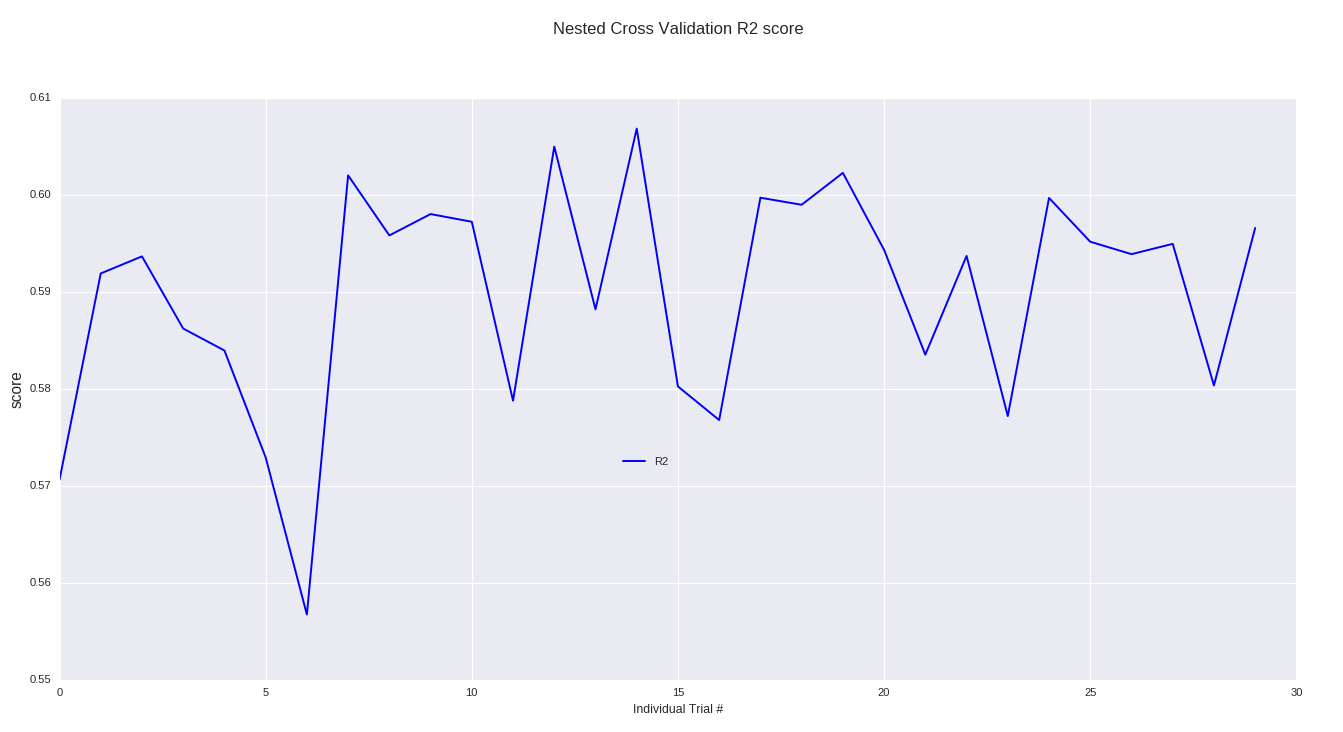
\includegraphics[scale=0.36]{R2.png}
	\caption{R2 score}
\end{center}
\end{figure*}
    

\begin{figure*}
\begin{center}
	\centering
	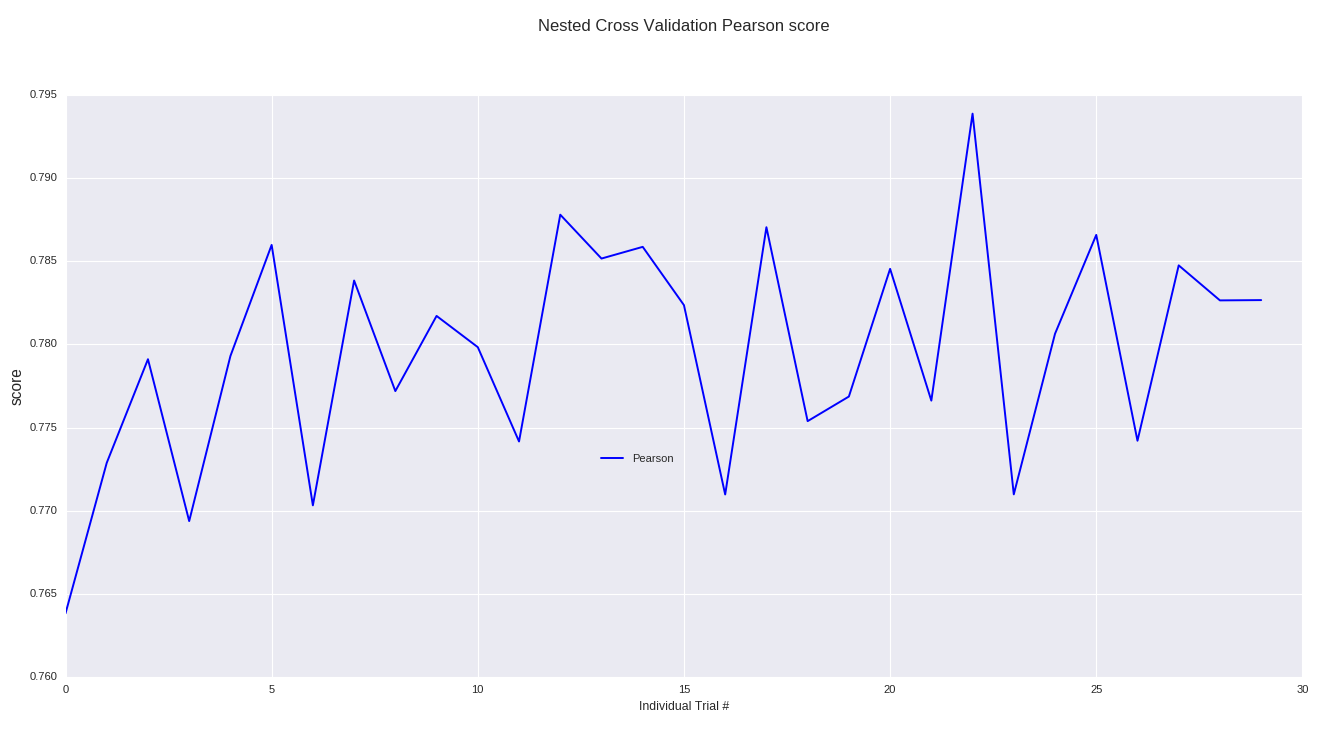
\includegraphics[scale=0.36]{Pearson.png}
	\caption{Pearson correlation score}
\end{center}
\end{figure*}

\begin{table}
\caption{Averaged scores}
\label{tab:narrow-table}
\begin{center}
\begin{tabular}{ccc}
\toprule
& R2 & Pearson\\
\midrule
score & 0.5898 & 0.7795 \\
\bottomrule
\end{tabular}
\end{center}
\end{table}

\subsection{Deep learning}


\newpage
\begin{figure}
\begin{center}
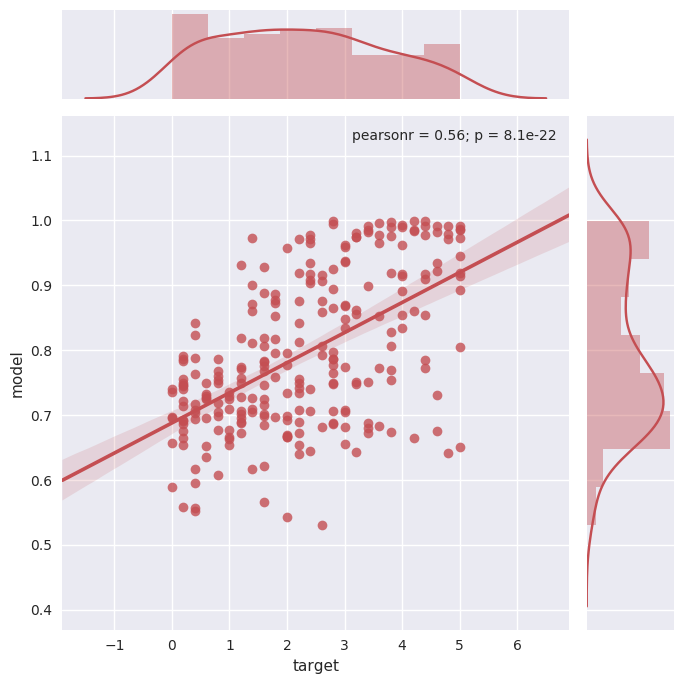
\includegraphics[width=\columnwidth]{only_2nd_layer.png}
\caption{Depiction of blabla}
\label{fig:lstm_2nd_layer}
\end{center}
\end{figure}



\section{Conclusion}

\bibliographystyle{tar2016}
\bibliography{tar2016}
\nocite{*}

\end{document}
